% Put labels, etc., on figures using PSTricks.
% Use dvips -E <file>.dvi -o <file>.eps to create encapsulated PostScript.
%
\documentclass[12pt]{article}
\usepackage{graphicx}
\usepackage{pstricks}
\pagestyle{empty}

\begin{document}
\rput(5,-5){
\rput(.1,-.1){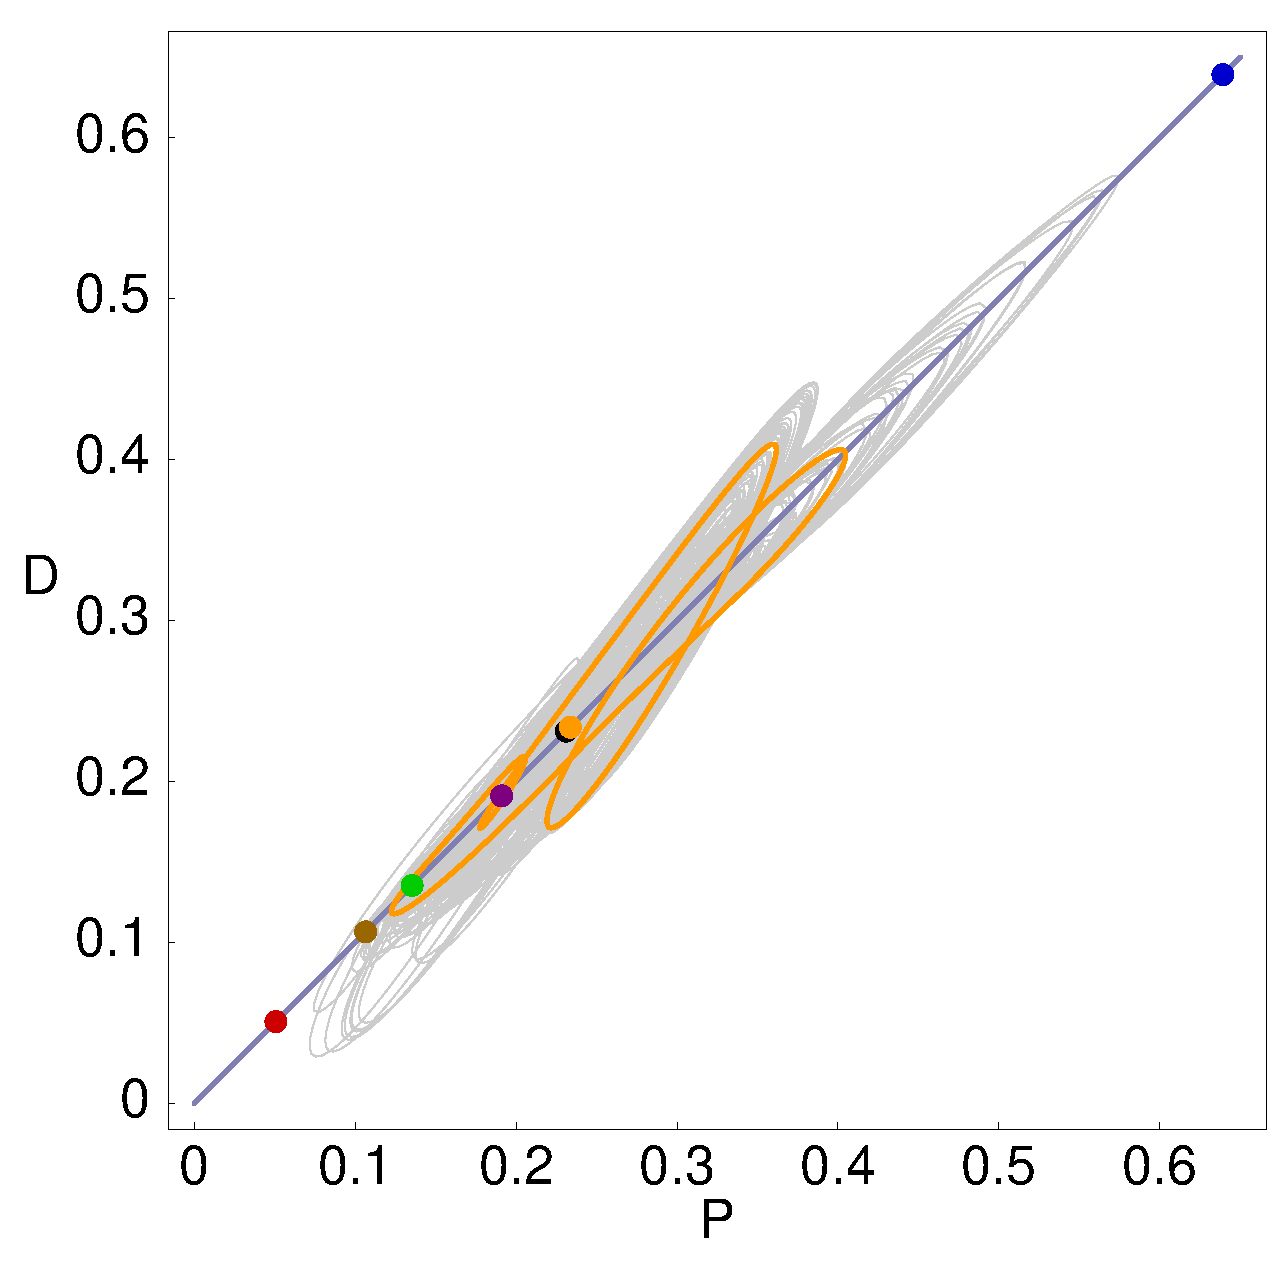
\includegraphics{../../rpo_ks/figs/energyBalancePlot.eps}}

\huge

\psframe*[linecolor=white](-6.5,6)(-5.5,7)
\psframe*[linecolor=white](6,-6.5)(7.2,-5.5)

\rput(10.1,8.9){E$_3$} \rput(-6.6,-5.9){E$_1$}

\psline[linewidth=2pt]{->}(-4.7,-3.6)(-3.9,-4.05)\rput(-5.2,-3.5){E$_2$}
\psline[linewidth=2pt]{->}(-5.3,-4.5)(-4.7,-4.9)\rput(-6.5,-4.5){TW$_{\pm1}$}
\psline[linewidth=2pt]{->}(-3.7,-2)(-2.3,-2.6)\rput(-5,-2.0){TW$_{\pm2}$}
\psline[linewidth=2pt]{->}(5.8,2)(5.1,3.9)\rput(6,1.5){``Turbulence''}
\psline[linewidth=2pt]{->}(3,-0.5)(1.05,-0.05)\rput(6,-0.5){$T\simeq 33\,, l\simeq 11$}
\psline[linewidth=2pt]{->}(-2,2.5)(-1.05,-1.4)\rput(-3,4){$T\simeq 33\,, l\simeq 11$,}\rput(-3,3){Time Average}
\psline[linewidth=2pt]{->}(-5,0)(-1.2,-1.6)\rput(-5,1.5){``Turbulence'',}\rput(-5.,0.5){Time Average}



% Use grid command below to place objects at specified coordinates.
% \psgrid[subgriddiv=1,griddots=10](-8,-8)(10,10)
}
\end{document}
